%\documentclass[a4paper,10pt]{jarticle}
%\documentclass[]{jarticle}
\documentclass[10pt]{jarticle}

%\usepackage{graphicx}
\usepackage[dvipdfmx]{graphicx}
\usepackage{eclbkbox} %breakbox用

%本文領域を広め(空白箇所マージン領域を小さめ)に設定
\setlength{\textwidth}{179mm}
\setlength{\textheight}{251mm}
\setlength{\topmargin}{-2cm}
\setlength{\oddsidemargin}{-1cm}
\setlength{\evensidemargin}{-1cm}

\begin{document}

\title{情報工学実験IIレポート(探索アルゴリズム1)}
\author{曜日&グループ番号: 月曜日&グループ2} %
\date{2015年12月11日}

\maketitle

\begin{abstract}
この骨組み(テンプレート)を利用する際には、
不要な箇所を削除した上で提出すること。
例えばこの要旨やコメント文の殆どは
「當間から学生へのコメント」であって、
「課題に対するレポート(報告書)」ではない。

このレポート(ファイル)は、「情報工学実験II・探索アルゴリズムその
1\cite{info2-search1}」の実験レポートの骨組みを例示している。
あくまでも例示であって、全てをこの通りに従う必要はないが、
指示された項目を含めた上で、
報告書として他者が読みやすいレポートとなるよう考慮すること。
\end{abstract}

\section*{グループメンバ}
(補足:レベル毎に \underline{全員が協力して実施} した上で、レベル毎にレポートをまとめる担当者を決め、全体を一つのレポートとして整理すること。分担方法も自由である。)
\begin{itemize}
	\item 145763C 仲村 大地: Level1.1, 2.1
	\item 145738B 西銘 明留: Level1.2, 1.3
	\item 145717K 泉川真理南: Level2.2, 3.0
	\item 145714E 豊美 玲 : Level2.3 
\end{itemize}

\section*{提出したレポート一式について}
レポート一式は
``\verb|shell:/net/home/teacher/tnal/2015-search1-mon/group2/|''
にアップロードした。
提出したファイルのディレクトリ構成は以下の通りである。

\vspace{+0.5cm}
(補足:必ず下記のように整理しろという指定ではない。
自分たちでやりやすいようにLevel毎に整理しても構わない)
\begin{breakbox}
\begin{verbatim}
./src/      # 作成したプログラム一式
./report/   # レポート関係ファイル.図ファイルを含む.
\end{verbatim}
\end{breakbox}

\newpage

\section{Leve l1: 最適化とは}
\subsection{Level 1.1: $B%3%s%T%e!<%?$H?M4V$N0c$$$r=R$Y$h(B}
\subsubsection{$B2]Bj@bL@(B}
$B%3%s%T%e!<%?$,?M4V$h$jF@0U$H$9$k%b%N!"$=$NH?BP$K?M4V$h$jITF@<j$N%b%N!"N><T$K$D$$$F(B2$B$D0J>e$N;kE@!JN)>l$d4QE@$J$I!K$r<($7!"9M;!$9$k!#(B

\subsubsection{$B9M;!(B}
\begin{itemize}
 \item $B;kE@(B1: hoge\\
$B%3%s%T%e!<%?$J$i$P!v!v$,2DG=$G$"$j1>!9(B
 \item $B;kE@(B2: fuga\\
$B?M4V$O!v!v$7$J$/$F$O$J$i$J$$$?$a1>!9(B
\end{itemize}

\subsection{Level 1.2: 住宅価格を推定するモデルについて}

\subsubsection{課題説明}

Housing Data Set\cite{housingdata}
におけるRM(平均部屋数)からMEDV(平均価格)を推定するた
めのモデルについて検討した。

\subsubsection{モデルへの入力}

入力=RM(平均部屋数)

\subsubsection{モデルにおける処理内容}

散布図からおおよその傾向を読み取った結果,\\
10*RM-40でMEDVを推定できるのではないかと考えた.

\subsubsection{モデルの出力}

出力=入力RMから推定されたMEDV(平均価格)\\
出力結果を以下の図で示す.緑の線でかかれたモデルが推定されたMEDVを表すものである.

\begin{figure}[ht]
 \begin{center}
  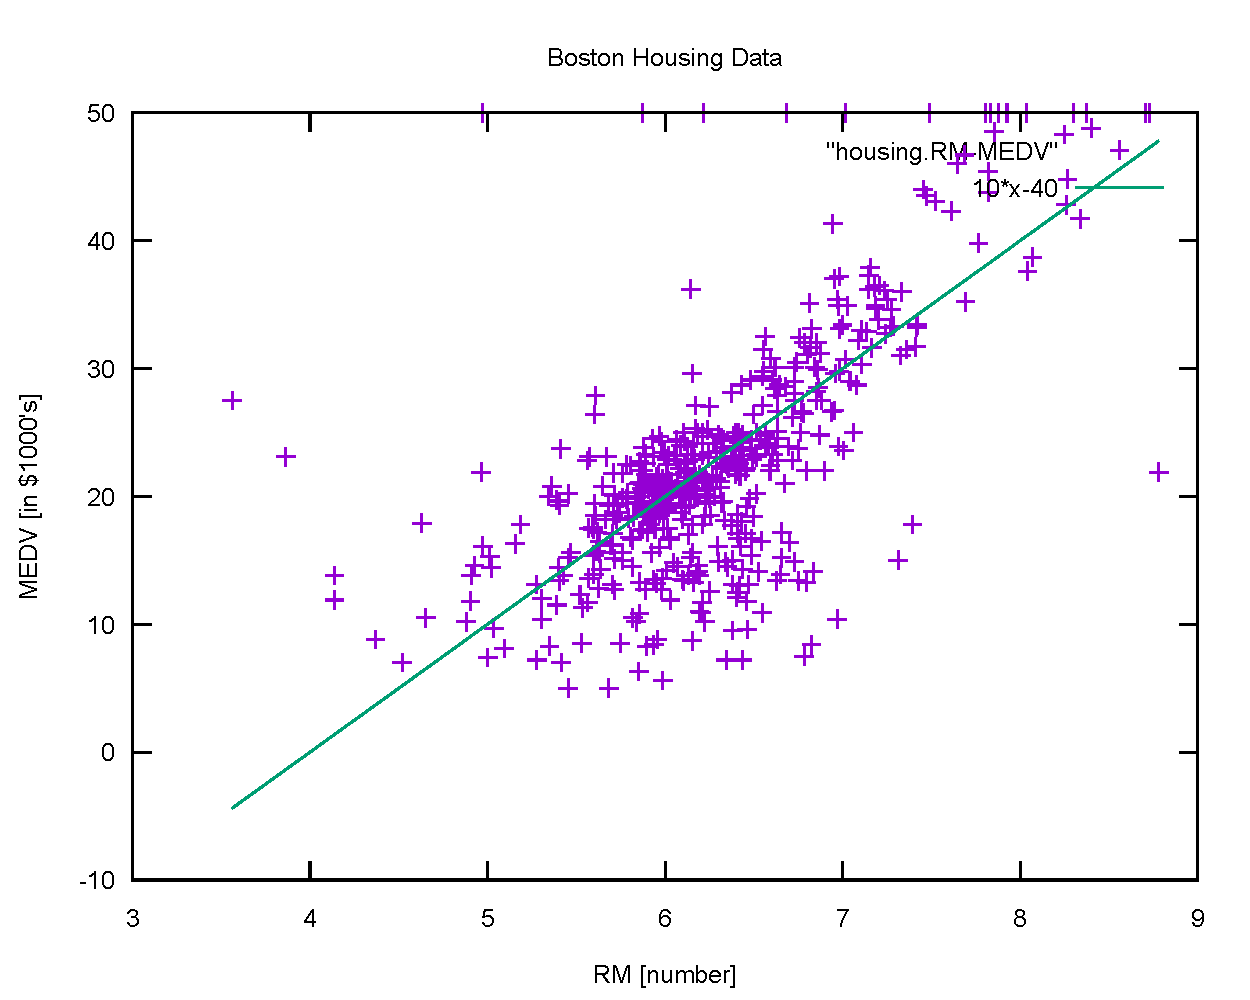
\includegraphics[width=10.0cm]{figs/level1.2/housing.pdf}
  \caption{探索初期値の変化}
 \end{center}
\end{figure}




\subsection{Level 1.3: モデルの良さを評価する方法について}

\subsubsection{課題説明}
Level 1.2 で検討したモデルの適切さを評価する指標について検討した。

\subsubsection{評価に用いる情報源}

RM(平均部屋数),MEDV(平均価格),Level1.2で推定されたMEDV

\subsubsection{評価手順}

RMとMEDVから,おなじRMのMEDVのデータからMEDVの平均値をとる.\\
この平均値と推定されたMEDVの差を比較する.

\subsubsection{評価に基づいた適切さを計る方法}

差が小さいほど適切なモデルである.

\newpage

\section{Level 2: 最急降下法による最適化}
\subsection{$B2]Bj@bL@(B}
3$B<oN`$NO"B34X?t(B$y=x^2$$B!"(B$z=x^2+y^2$$B!"(B$y=-x \times cos(x)$$B$K$D$$$F!"(B
$B:G5^9_2<K!$NE,MQ$rDL$7$FC5:w5sF0$r4Q;!$7$?!#(B
$B0J2<$G$O$^$:6&DLItJ,$G$"$k:G5^9_2<K!$NC5:w<jB3$-$K$D$$$F!"(B
$B%U%m!<%A%c!<%H$rMQ$$$F2r@b$9$k!#(B
$B$=$N8e!"(B3$B<oN`$N4X?tKh$K%W%m%0%i%`$NJQ992U=j!"(B
$B4Q;!0U?^4Q;!J}K!!"4Q;!7k2L!"9M;!$K$D$$$F@bL@$9$k!#(B


\subsection{Level 2$B6&DLItJ,(B}
$B!JJdB-!'(BLevel2.1, 2.2, 2.3 $B$K$O6&DL$9$kItJ,$,B?$$$?$a!"(B
$B6&DLItJ,$OFHN)$7$FJs9p$9$k$HNI$$$G$7$g$&!K(B

\subsubsection{$BC5:w$N<jB3$-!J6&DLItJ,!K(B}

\subsubsection{$B%U%m!<%A%c!<%H!J6&DLItJ,!K(B}
$B!J<jB3$-$H%U%m!<%A%c!<%H$O$^$H$a$F0l$D$N@a$K$7$F$b9=$$$^$;$s!K(B

 %共通部分の結果及び考察
\subsection{Level2.1: $y=x^2$ $B$K$D$$$F(B}
\subsubsection{$B%W%m%0%i%`%=!<%9!JJQ99ItJ,!K(B}
\subsubsection{$B4Q;!0U?^$H4Q;!J}K!(B}
\subsubsection{$B<B9T7k2L(B}
\subsubsection{$B9M;!(B}


\subsection{Level2.2: $z=x^2 + y^2$ について}
\subsubsection{プログラムソース(変更部分)}
\begin{breakbox}
\begin{verbatim}
行数 変更点
32 z=x*x+y*y;
44  z_dx = 2*x*z_dx;
56 z_dy = 2*y*z_dy;
\end{verbatim}
\end{breakbox}

\subsubsection{観察意図と観察方法}

学習係数が探索挙動に及ぼす影響を確認するために,seed値とalpha値を変更し観察を行う.\\

\begin{enumerate}
\item alpha値を固定してseed値を変更する.\\
alpah値は0.1で固定,seed値は1~10,1000刻みの1000~10000とする.
\item seed値を固定してalpha値を変更する.\\
seed値は1で固定,alpha値は0.1~0.9とする.
\end{enumerate}

\subsubsection{実行結果}


1.seed値を変更したときのstep数.\\
step数に多少の変化がみられたものの,劇的な変化ではなかった.\\\\

2.alpha値を変更したときのstep数.\\


alpha値を変更したことにより,step数に大きな変化がみられた.\\
特にalpha値を0.1から0.2に変化させたときにstep数の大幅な減少がみられる.\\\\

\begin{table}[htb]
 \begin{center}
  \caption{alpha値を変更したときのstep数の変化}
  \label{table:level3}
  \begin{tabular}[htb]{r|l} \hline
   alpha値 &  step数\\ \hline \hline
   0.1 &  686\\ \hline
   0.2 & 184 \\ \hline
   0.3 & 82 \\ \hline
   0.4 & 45 \\ \hline
   0.5 & 26 \\ \hline
   0.6 & 16 \\ \hline
   0.7 & 19 \\ \hline
   0.8 & 16 \\ \hline
   0.9 & 40 \\ \hline \hline

  \end{tabular}
 \end{center}
\end{table}


またstep数が変化すると探索ステップ数あたりの目的関数推移図にも変化が生じることがわかった.\\

\begin{figure}[ht]
 \begin{center}
  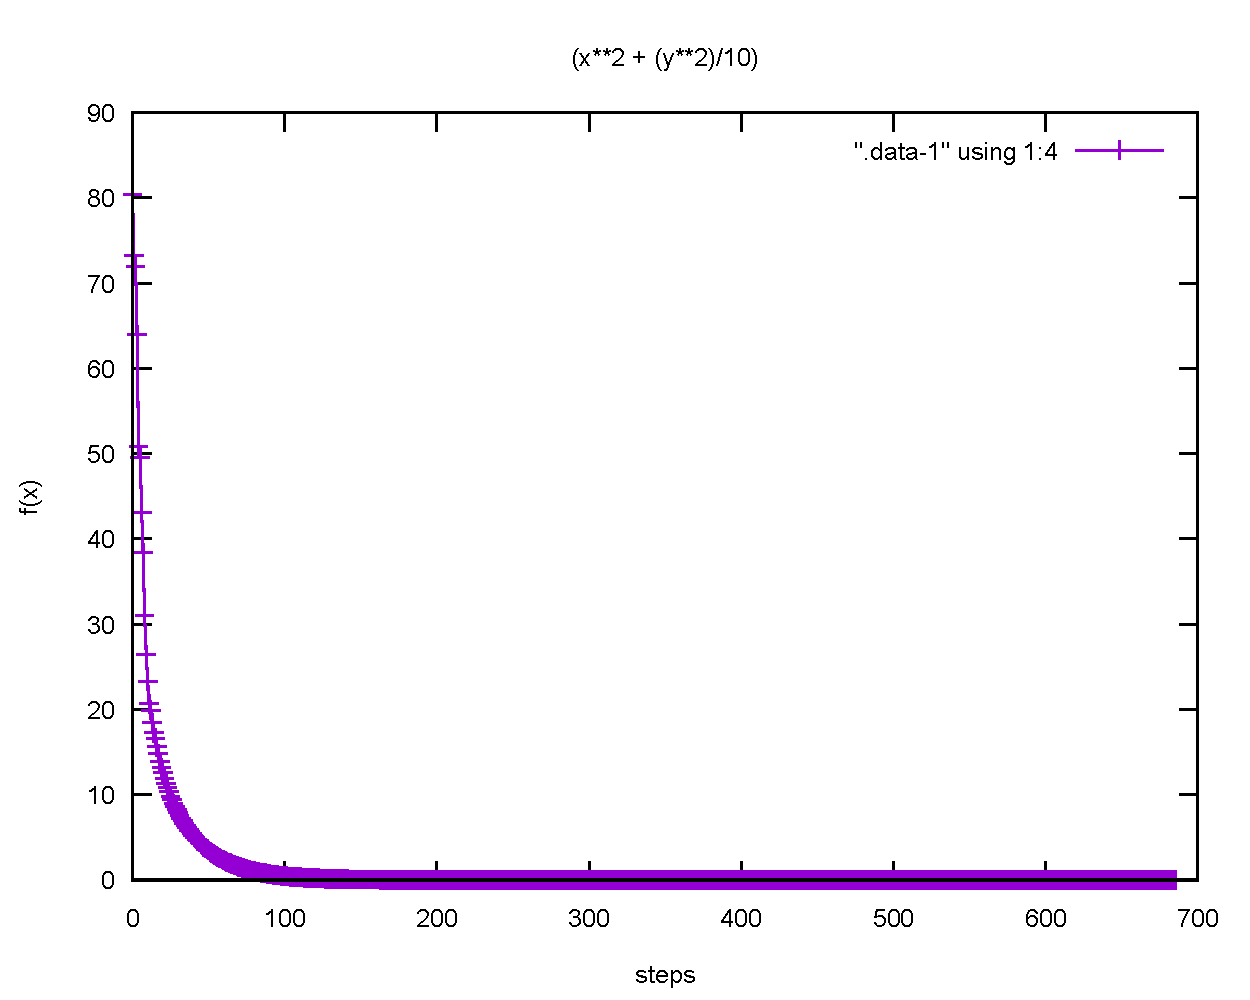
\includegraphics[width=10.0cm]{figs/level2.2/sim-1-2.pdf}
  \caption{alpha値0.1のときの推移図}
	\label{step_alpha}
 \end{center}
\end{figure}

\begin{figure}[ht]
 \begin{center}
  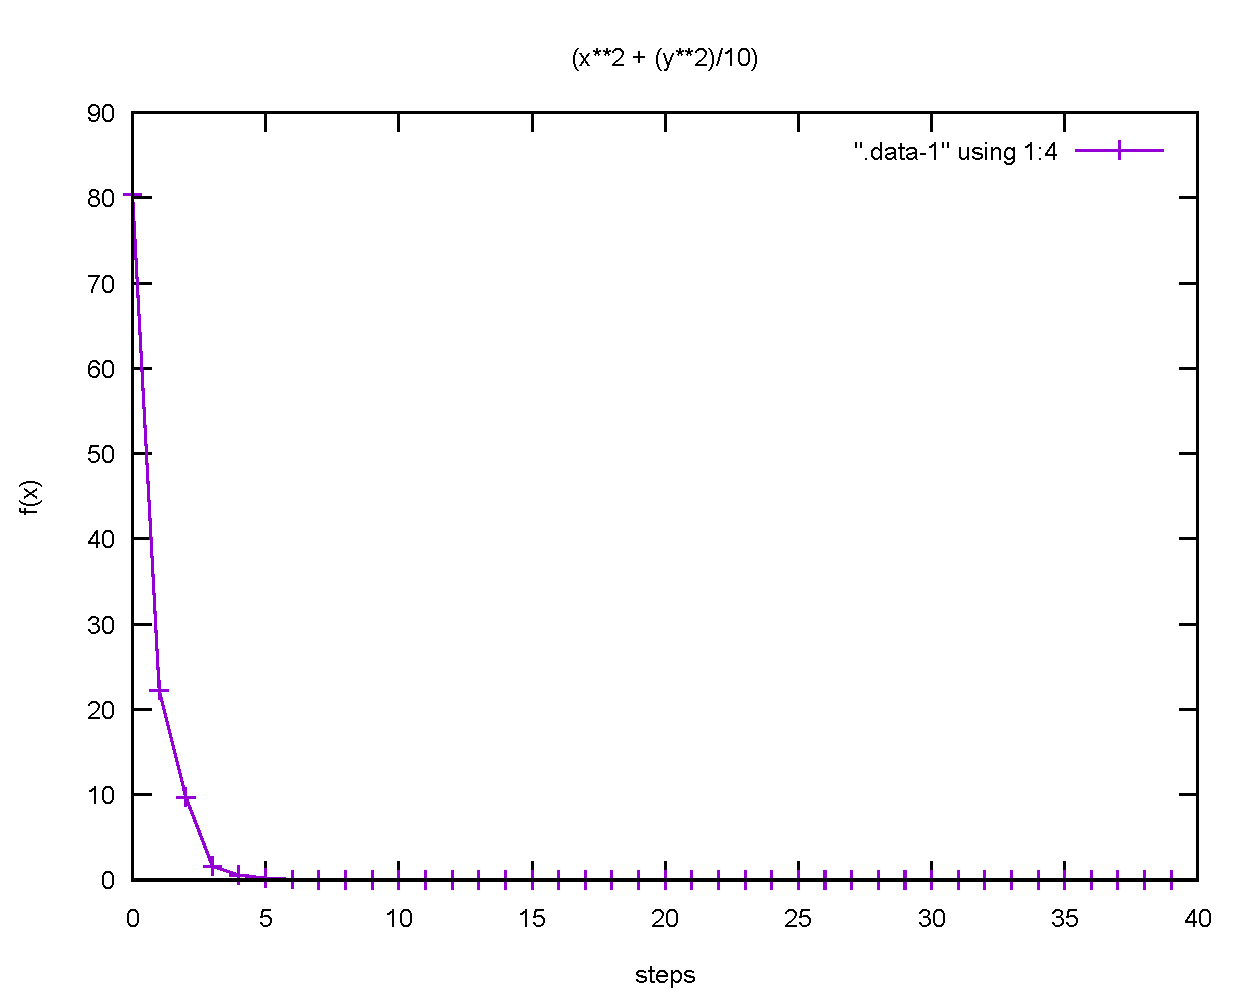
\includegraphics[width=10.0cm]{figs/level2.2/sim-1.pdf}
  \caption{alpha値0.9のときの推移図}
	\label{step_alpha}
 \end{center}
\end{figure}

alpha値0.1(step数が多い)ときのほうが図がなめらかである.

\subsubsection{考察}

学習係数を変化させることによりstep数を減らすことができた.探索回数が減ることにより効率はあがったと考える.\\
しかし,探索ステップ数あたりの目的関数推移図を見ると,step数が多いほうが探索点が最適解にたどりついたより正確な地点を知ることができると考える.




\subsection{Level2.3: $y=-x*cos(x)$ について}
\subsubsection{プログラムソース(変更部分)}
\subsubsection{観察意図と観察方法}
\subsubsection{実行結果}
\subsubsection{考察}



\newpage

\section{Level 3: 最急降下法が苦手とする状況}
\subsection{課題説明}

最急降下法が苦手とする状況についてその理由を解説し,
検討した改善方法について解説する.

\subsubsection{原因}

「山(谷)」の数は一つにも関わらず最も勾配の高い方向に移動するため,一直線に谷には向かわずジグザグ移動してしまい,効率的ではない.

\subsubsection{改善方法}

・複数の初期値から探索を行いより短い探索で解にたどり着ける初期値を探す.\\
最適解の近傍に初期値を設定することができれば,余計な探索を減らすことができると考えた.
最適解のx軸方向の直線上に近い場所に初期値を設定することができれば,一直線に谷に向かうことも可能となる.\\\\


・また収束速度を安定させる手法として,前回得られた勾配ベクトルと今回得られた勾配ベクトルの符号の変化によって刻み幅の調整をする方法がある.符号が反転したときに刻み幅を小さくし,符号が等しいときに刻み幅を大きくすることで安定して収束する.





 %課題説明+提案解説

\vspace{+1.0cm}
(補足:参考文献は thebibliography 環境を使って列挙し、
本文中で適切な箇所で引用するようにしましょう。
例えば下記文献は、アブストラクトやLevel 4で引用しています)
\begin{thebibliography}{99}
\bibitem{info2-search1}
情報工学実験2: 探索アルゴリズムその1(當間)\\
\verb|http://www.eva.ie.u-ryukyu.ac.jp/~tnal/2015/info2/search1/|
\bibitem{housingdata}
Housing Data Set\\
\verb|http://archive.ics.uci.edu/ml/datasets/Housing|
\end{thebibliography}

\end{document}
